\documentclass[11pt,a4paper]{book}
\textwidth 170 mm
\textheight 250 mm
\topmargin -15 mm
\oddsidemargin -5 mm
\evensidemargin -5 mm

\newcounter{ProblemNo}
\setcounter{ProblemNo}{0}
\def\tempID{0}
%\def\UndAns{} %% <-------------- Uncomment in final version!!
\def\UndAns{\underline}
\def\UndAns{\underline}
\newcommand{\ZOdg}[1]{}
\def\text{}
%\def\dfrac{\displaystyle\frac}

\usepackage{amsfonts,amssymb,amsmath}
\usepackage{graphicx}
\DeclareGraphicsExtensions{.pdf,.PDF,.png,.PNG} % prefer pdf to png
\usepackage{etoolbox}
\usepackage{sidepicture}
\newcommand{\problemID}[3]{\def\tempID{#1 (#3)}\ignorespacesafterend}
%\newcommand{\problemID}[3]{\def\tempID{#1}\noindent{\bf #1, #2}\par}
%\newcommand{\problemID}[3]{\def\tempID{#3: \##1}\par}
%\newcommand{\problemRating}[3]{{\bf #1, #2, #3}\par}
%\newcommand{\problemID}[3]{\def\tempID{\# #1}\par}
%\newcommand{\problemRating}[3]{}
%\newcommand{\xProblem}[8]{#1\par (A) #2\quad (B) #3\quad  (C) #4\quad  (D) #5\quad (E) #6\par Correct: #7\bigskip\bigskip\par }

%\usepackage{xcolor}
%\usepackage{everypage}
%\usepackage[absolute]{textpos}
%\usepackage{rotating}
%\AddEverypageHook{\begin{textblock*}{2.5cm}(0.7cm,5cm)\begin{turn}{90}{\color{red}\Huge\sc Solutions included - do not use for contest}\end{turn}\end{textblock*}}

\newcommand{\Problem}[9]
{%\newpage
%\noindent\addtocounter{ProblemNo}{1}{\bf\arabic{ProblemNo}.\hspace{3pt}~}%
\noindent\addtocounter{ProblemNo}{1}{\bf\tempID.\hspace{3pt}~}%
\edef\answer{{#7}}\def\SettingMode{#8}%
\def\VLine{\vrule height14pt width0pt\quad}#1\nopagebreak\vspace{1ex}\newline%
\VLine\expandafter\ifstrequal\answer{A}{\UndAns{(\rlap{\bf A}\phantom{\bf C})}\ZOdg{A}}{(\rlap{\bf A}\phantom{\bf C})}\nolinebreak\hspace{3pt}%
\ifnum\SettingMode=3{#2}\else\rlap{#2}\fi\quad\ifnum\SettingMode=3\newline\VLine\else\hfil\fi%
\expandafter\ifstrequal\answer{B}{\UndAns{(\rlap{\bf B}\phantom{\bf C})}\ZOdg{B}}{(\rlap{\bf B}\phantom{\bf C})}\nolinebreak\hspace{3pt}%
\ifnum\SettingMode=3{#3}\else\rlap{#3}\fi\quad\ifnum\SettingMode=2\newline\VLine\else\ifnum\SettingMode=3\newline\VLine\else\ifnum\SettingMode=6{\phantom{({\bf C})}\quad\hspace{6pt}\hfil\hfil\newline\VLine}\else\hfil\fi\fi\fi%
\expandafter\ifstrequal\answer{C}{\UndAns{(\rlap{\bf C}\phantom{\bf C})}\ZOdg{C}}{({\bf C})}\nolinebreak\hspace{3pt}%
\ifnum\SettingMode=3{#4}\else\rlap{#4}\fi\quad\ifodd\SettingMode\newline\VLine\else\hfil\fi%
\expandafter\ifstrequal\answer{D}{\UndAns{(\rlap{\bf D}\phantom{\bf C})}\ZOdg{D}}{(\rlap{\bf D}\phantom{\bf C})}\nolinebreak\hspace{3pt}%
\ifnum\SettingMode=3{#5}\else\rlap{#5}\fi\quad\ifnum\SettingMode>1\ifnum\SettingMode<6\newline\VLine\else\hfil\fi\else\hfil\fi%
\expandafter\ifstrequal\answer{E}{\UndAns{(\rlap{\bf E}\phantom{\bf C})}\ZOdg{E}}{(\rlap{\bf E}\phantom{\bf C})}\nolinebreak\hspace{3pt}%
\ifnum\SettingMode=3{#6}\else\rlap{#6}\fi\quad\ifnum\SettingMode=1\hfil\phantom{({\bf C})}\fi\hspace{3pt}\hfil\par\vspace{2ex}\par\noindent{\sc Solution: }#9\bigskip}


\def\TheHead{Cadet Finalized}
\makeatletter
\def\ps@pKSF{
\def\@oddfoot{\hfill{\rm \thepage}\hfill}\def\@evenfoot{\hfill{\rm \thepage}\hfill}
\def\@oddhead{\hfill{\em \TheHead}\hfill}\def\@evenhead{\hfill{\em \TheHead}\hfill}
}
\makeatother 
\pagestyle{pKSF}

\begin{document}

\noindent{\large\bf Cadet}\bigskip

\noindent\fbox{3 points}\bigskip

\NSidePictureEPS{C01-6}{\problemID{1}{20227}{Germany}%
\problemRating{C}{3}{G}%
\Problem{Which of the following strings cannot be transformed into the string on the right without cutting?}
{
\includegraphics{C01-1}}{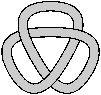
\includegraphics{C01-2}}{
\includegraphics{C01-3}}{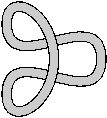
\includegraphics{C01-4}}{
\includegraphics{C01-5}}
{B}{0}
{Only for B, two rings are formed that must pass through each other and it is impossible to do this without cutting the string.}}

\NSidePictureEPS[scale=0.7]{C02-8}{\problemID{2}{20228}{Slovenia}%
\problemRating{C}{3}{G}%
\Problem{A shape is made of equal-sized pentagonal tiles. Which of the following tiles can be placed in the space in the shape to produce two closed curves?}
{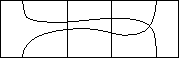
\includegraphics[scale=0.7]{C02-1}}{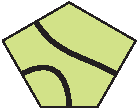
\includegraphics[scale=0.7]{C02-2}}{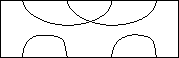
\includegraphics[scale=0.7]{C02-3}}{
\includegraphics[scale=0.7]{C02-4}}{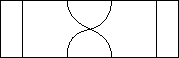
\includegraphics[scale=0.7]{C02-5}}
{C}{1}
{Note that all tiles are rotated by $180^\circ$.
No other rotation can make the tile fit as the pentagonal tile has exactly two right angles.
\newline
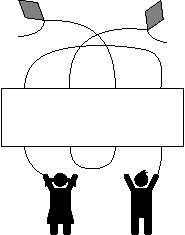
\includegraphics{C02-6}}}

\NSidePictureEPS{C03-1}{\problemID{3}{20229}{Spain}%
\problemRating{C}{3}{G}%
\Problem{The first diagram shows a rhombus. The area of the first diagram is increased by adding two right-angled triangles, as shown. By what percentage has the area increased?}
{$20\%$}{$25\%$}{$30\%$}{$40\%$}{$50\%$}
{E}{1}
{The initial figure can be divided into four right triangles of the same area, and the initial figure into six triangles, thus the proportion in $6/4$, that is $3/2=1.5$, therefore it has increased by $50\%$.\newline
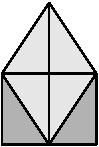
\includegraphics{C03-2}}}

\problemID{4}{20230}{Uganda}%
\problemRating{C}{3}{N}%
\Problem{What is the value of $\dfrac{20 \times 24}{2 \times 0+2 \times 4}?$}
{$12$}{$30$}{$48$}{$60$}{$120$}
{D}{0}
{$\frac{20\times24}{2\times0+2\times4}=\frac{20\times24}{0+8}=\frac{20\times3\times8}{8}=20\times3=60$}

\NSidePictureEPS{C05-1}{\problemID{5}{20231}{Germany}%
\problemRating{C}{3}{G}%
\Problem{Julio cuts off the four corners of a regular tetrahedron, as shown. How many corners does the shape that remains have?}
{8}{9}{11}{12}{15}
{D}{1}
{A tetrahedron has four corners. Three sides meet at each vertex. Every cut corner therfor gives three new corners. So if all four old corners are cut off, $4 \times 3=12$ new corners are created.}}

\NSidePictureEPS{C06-1}{\problemID{6}{20232}{Netherlands}%
\problemRating{C}{3}{N}%
\Problem{Ria has three counters marked 1, 5 and 11, as shown.  She wants to place them side by side to make a four-digit number. \newline
How many different four-digit numbers can she make?}
{$3$}{$4$}{$6$}{$8$}{$9$}
{B}{0}
{You can make 1511, 1115, 5111 and 1151. Notice that, normally you can make $3\cdot2\cdot1=6$ numbers, but when 1 and 11 are next to each other, the order is not important, so you lose $2$ possibilities.}}

\problemID{7}{20233}{Switzerland}%
\problemRating{C}{3}{L}%
\Problem{A fruit bowl contains five types of fruit: 

\includegraphics{C07-1},

\includegraphics{C07-2},

\includegraphics{C07-3},

\includegraphics{C07-4} and

\includegraphics{C07-5}.
Al likes 
\includegraphics{C07-1}. Bok likes 
\includegraphics{C07-1}, 
\includegraphics{C07-3}, 
\includegraphics{C07-4} and 
\includegraphics{C07-5}. Cam likes 
\includegraphics{C07-2}, 
\includegraphics{C07-3}, 
\includegraphics{C07-4} and 
\includegraphics{C07-5}. Don likes 
\includegraphics{C07-1}, 
\includegraphics{C07-2} and 
\includegraphics{C07-3}.  Eva likes 
\includegraphics{C07-1} and 
\includegraphics{C07-3}.

The fruit is shared so that everyone gets a different type of fruit and everyone gets a type of fruit that they like.\newline
Who gets 
\includegraphics{C07-3}?}
{Al}{Bok}{Cam}{Don}{Eva}
{E}{0}
{If we want that everyone gets the fruit she/he likes then Al gets the apple and Eva gets the cherries. \newline \includegraphics{C07-6}}

\problemID{8}{20234}{Ukraine}%
\problemRating{C}{3}{N}%
\Problem{The weight restriction notice for an elevator says it can carry either 12 adults or 20 children.  According to the weight restrictions, what is the largest number of children that can ride in the elevator with nine adults?}
{3}{4}{5}{6}{8}
{C}{0}
{We need to determine how many children can be in the elevator instead of $12 - 9 = 3$ adults.

If instead of 12 adults there can be 20 children,

then instead of four times less adults there can be four times less children, i.e. $20 : 4 = 5$}

\NSidePictureEPS{C09-1}{\problemID{9}{20235}{Australia}%
\problemRating{C}{3}{N}%
\Problem{Four different positive integers are placed on a grid and then covered
 up.  The products of the integers in each row and in each column are shown in the diagram. What is the sum of the four integers?}
{$10$}{$12$}{$13$}{$14$}{$15$}
{C}{1}
{In the top row, we either have a 2 and a 3, or a 1 and a 6.  If we
 place the 2 in the top left square, we will need to repeat a 2 in
 the bottom left square so this is not possible.  If we place a 3 or
 a 6 in the top left square, it gives a fraction in the bottom left.

 Hence, we must place a 1 in the top left square.  From here, we can
 fill in the whole grid as follows:
\newline
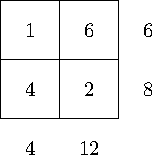
\includegraphics{C09-2}
\newline
Alternative solution: In the top left square we must write a common divisor of 4 and 6, it may be only 1 or 2. If we write  the 2 in the top left square, we will need to repeat a 2 in the bottom left square so this is not possible. So, it remains only 1 for the top left square. From here, we can fill in the whole grid as follows: \newline
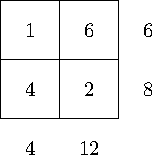
\includegraphics{C09-2}}}

\NSidePictureEPS[scale=0.7]{C10-1F}{\problemID{10}{20236}{Portugal}%
\problemRating{C}{3}{A}%
\Problem{The length of a set of four well-parked and fitted supermarket trolleys is 108 cm. The length of a set of ten well-parked and fitted supermarket trolleys is 168 cm.  What is the length of a single supermarket trolley?}
{60 cm}{68 cm}{78 cm}{88 cm}{90 cm}
{C}{0}
{The difference in length between 4 trolleys and 10 trolleys equals $60\,\mathrm{cm}$. Adding $10-4=6$ trolleys means adding 60 cm. So, adding one extra trolley means adding $60\,\mathrm{cm}:6=10\,\mathrm{cm}$  of length. This means that four trolleys minus the extra length of three trolleys $= 108\,\mathrm{cm} - 3 \times 10\,\mathrm{cm} =78\,\mathrm{cm}$. So the length of one trolley is $78\,\mathrm{cm}$.
\newline Alternative solution
\newline
Let the length of one trolley equal $x\, \mathrm{cm}$ and let the left part of the first (from left) trolley, which is not covered by other trolleys, equal $y\, \mathrm{cm}$. The length of a set of four well-parked trolleys consists of three parts y of the first three trolleys and the length $x$ of the forth trolley. Thus, $3y+x=108$. Analogously, for ten trolleys we have $9y+x=168$. It follows that $6y=168-160= 60$ and $y=10\,\mathrm{cm}$. The length of one trolley is equal to $x=108-3y=78 \,\mathrm{cm}$.}}

\noindent\fbox{4 points}\bigskip

\NSidePictureEPS[yoffset=-3.5ex]{C11-1}{\problemID{11}{20237}{Germany}%
\problemRating{C}{4}{G}%
\Problem{Carina baked a cake and cut it into ten equal pieces.
She ate one piece and then arranged the remaining pieces evenly, as shown.
What is the size of the angle between any two pieces?}
{$5^\circ$}{$4^\circ$}{$3^\circ$}{$2^\circ$}{$1^\circ$}
{B}{0}
{The angle of each piece  is $\dfrac{360^\circ}{10} = 36^\circ$. There are 9 gaps. Hence, the angle of each gap is $\dfrac{36^\circ}{9} = 4^\circ$.}}

\problemID{12}{20238}{Germany}%
\problemRating{C}{4}{L}%
\Problem{Werner can make a $4 \times 4$ square, where the sum of the numbers in all four rows and all four columns is the same, from the three pieces shown 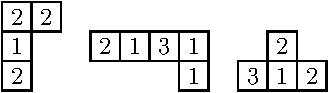
\includegraphics{C12-1} and one further piece.
Which of the following pieces is needed to complete his square?}
{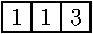
\includegraphics{C12-2}}{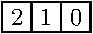
\includegraphics{C12-3}}{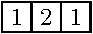
\includegraphics{C12-4}}{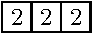
\includegraphics{C12-5}}{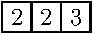
\includegraphics{C12-6}}
{A}{0}
{One of the given pieces has a row of four numbers with sum $2 + 1 + 3 + 1 = 7$.  Therefore the sum of the numbers in the whole square is $4 \times 7 = 28$.  The sums of the numbers on the three pieces are 7, 8 and 8 and hence a piece where the numbers sum to $28 - 7 - 8 - 8 = 5$ is required.  Of the options given, the only one with a sum of 5 is A.  The diagram below shows how these four pieces fit together to make the square.\newline
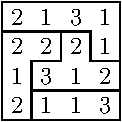
\includegraphics{C12-7}}

\NSidePictureEPS[yoffset=-5.5ex]{C13-2}{\problemID{13}{20239}{Greece}%
\problemRating{C}{4}{G}%
\Problem{A square has side-length $10\ \textup{m}$. It is divided into parts by three straight line segments, as shown. The areas of the two shaded triangles are $A$ and $B$.  What is the value of $A - B$?}
{$0\ \textup{m}^2$}{$1\ \textup{m}^2$ }{$2\ \textup{m}^2$}{$5\ \textup{m}^2$ }{$10\ \textup{m}^2$}
{A}{0}
{Areas $A+C$ and $B+C$ are equal since both are half the square. So $A-B = (A+C)-(B+C) = 0$.\newline
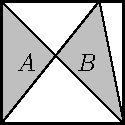
\includegraphics{C13-1}}}

\problemID{14}{20240}{United Kingdom}%
\problemRating{C}{4}{N}%
\Problem{Paula the penguin goes fishing every day and always brings back twelve fish for her two chicks.\newline
Each day, she gives the first chick she sees seven fish and gives the second chick five fish, which they eat.\newline
In the last few days one chick has eaten 44 fish.\newline
How many has the other chick eaten?}
{34}{40}{46}{52}{58}
{D}{0}
{The only way a chick can have eaten 44 fish in total is to have eaten 5 fish six times and 7 fish twice.  Therefore it had eaten fish on 8 days.  The number of fish Paula brought back on those 8 days was $8\times 12 = 96$.  Hence the number of fish eaten by the second chick was $96 - 44 = 52$.}

\NSidePictureEPS{C15-1}{\problemID{15}{20241}{Brazil}%
\problemRating{C}{4}{G}%
\Problem{Johan had a large number of identical cubes. He made the structure on the right by taking a single cube and then sticking another cube to each face.  He wants to make an extended structure in the same way so that each face of his original structure will have a cube stuck to it.  How many extra cubes will he need to complete his extended structure?}
{18}{16}{14}{12}{10}
{A}{0}
{There are 30 faces to cover. Adding a cube into one of the "angles" about one edge of the innermost cube of the structure covers 2 (inner) faces at the same time. There are 12 edges of this innermost cube, hence with 12 cubes you cover these 24 inner faces. To cover the outermost faces you need 6 more cubes, hence 18 cubes altogether.}}

\problemID{16}{20242}{Austria}%
\problemRating{C}{4}{N}%
\Problem{A kangaroo jumps up a mountain and then jumps back down along the same route. It covers three times the distance with each downhill jump as it does with each uphill jump.  Going uphill, it covers 1 metre per jump.  In total, the kangaroo makes $2024$ jumps.  What is the total distance, in metres, that the kangaroo jumps?}
{506}{1012}{2024}{3036}{4048}
{D}{0}
{Let $u$ denote the number of uphill jumps and $d$ the number of downhill jumps.  Since the kangaroo covers three times the distance with each downhill jump as it does with each uphill jump, it will make three times as many uphill jumps as it does downhill jumps.  Therefore $u = 3d$.  Since we are told that $u + d = 2024$, we have $3d + d = 2024$ which has solution $d = 506$.  Therefore the total distance, in metres, that the kangaroo jumps is $506 \times 3 + 3\times 506 \times 1 = 3036$.}

\NSidePictureEPS[yoffset=-5.5ex]{C17-1}{\problemID{17}{20243}{Netherlands}%
\problemRating{C}{4}{A}%
\Problem{Gerard cuts a large rectangle into four smaller rectangles.
The perimeters of three of these smaller rectangles are 16, 18 and 24, as shown in the diagram.\newline
What is the perimeter of the fourth small rectangle?}
{$8$}{$10$}{$12$}{$14$}{$16$}
{B}{1}
{From the diagram, it can be seen that the perimeter of the rectangle in the top left and the perimeter of the rectangle in the bottom right together are equal to the perimeter of the large rectangle.  The same argument is true for the perimeter of the rectangle in the bottom left and the perimeter of the rectangle in the top right.  Therefore $24+{?}=18+16$ and hence $?=10$.}}

\problemID{18}{20244}{Hungary}%
\problemRating{C}{4}{A}%
\Problem{Water makes up 80 percent of the mass of fresh mushrooms.  However, water makes up only 20 percent of the mass of dried mushrooms. By what percentage does the mass of the mushroom decrease during drying?}
{60}{70}{75}{80}{85}
{C}{0}
{Consider 100 grams of fresh mushrooms.  Since 80 \% of this is water, the remainder has a mass of 20 grams.  When dried, this 20 grams now represents 80\% of the total mass and so the 20\% that is water has a mass of 5 grams.  Therefore the total mass of the dried mushrooms is 25 grams and hence the decrease is 75 grams or 75\% of the original mass.  
\newline Algebraic Solution: \newline
Let the mass of the water in the dried mushrooms be $X$ grams.  Since this represents 20\% of the total mass, the mass of the remainder four times as much and so is $4X$ grams.  However, this $4X$ grams represents only 20\% of the mass of fresh mushrooms and hence the mass of water in the fresh mushrooms is four times as much and so is $16X$ grams.  Therefore the percentage decrease in the mass is $\dfrac{(16X + 4X) - (4X + X)}{(16X + 4X)} \times 100 = \dfrac{15X}{20X} \times 100 = 75$}

\problemID{19}{20245}{Finland}%
\problemRating{C}{4}{N}%
\Problem{Teri the tiler is planning to make a large, square mosaic floor with a repeating pattern, using hexagonal and triangular tiles, arranged as shown in the diagram. \newline
\centerline{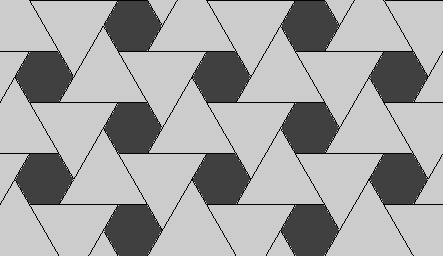
\includegraphics{C19-1}}\newline
She thinks she will use 3000 hexagonal tiles to make the whole floor.  Approximately, how many triangular tiles will she need?}
{1000}{1500}{3000}{6000}{9000}
{D}{0}
{Each hexagon is surrounded by six triangles, and every triangle touches three hexagons. There are $6/3=2$ triangles per hexagon, so approximately 6000 altogether.}

\problemID{20}{20246}{Vietnam}%
\problemRating{C}{4}{L}%
\Problem{Nine cards numbered from 1 to 9 were placed facedown on the table.  Aleksa, Bart, Clara and Deindra each picked up two of the cards.  Aleksa said "My numbers add up to 6". 
Bart said "The difference between my numbers is 5". 
Clara said "The product of my numbers is 18". 
Deindra said "One of my numbers is twice the other one". 
All four made a true statement.
Which number was left on the table?}
{1}{3}{6}{8}{9}
{E}{0}
{Since all four made a true statement, the numbers on Aleksa's cards were 1 and 5 or 2 and 4, the numbers on Bart's cards were 1 and 6, 2 and 7, 3 and 8 or 4 and 9, the numbers on Clara's cards were 2 and 9 or 3 and 6 and the numbers on Deindra's cards were 1 and 2, 2 and 4, 3 and 6 or 4 and 8. \newline
Suppose the numbers on Aleksa's cards were 2 and 4. Then the numbers on Clara's cards could only be 3 and 6.  However, this would not leave any possible cards for Deindra.  Therefore the numbers on Aleksa's cards were 1 and 5.\newline
Now suppose the numbers on Clara's cards were 2 and 9.  Then the numbers on Deindra's cards could only be 3 and 6.  However, this would not leave any possible cards for Bart.  Therefore the numbers on Clara's cards were 3 and 6.\newline
Finally suppose the numbers on Bart's cards were 4 and 9.  However this leaves no possible cards for Deindra.  Therefore the numbers on Bart's cards were 2 and 7, leaving cards numbered 4 and 8 for Deindra.  Hence the card numbered 9 is left on the table.}

\noindent\fbox{5 points}\bigskip

\problemID{21}{20247}{Finland}%
\problemRating{C}{5}{L}%
\Problem{The digits 0 - 9 can be drawn with horizontal and vertical segments, as shown. \newline
\centerline{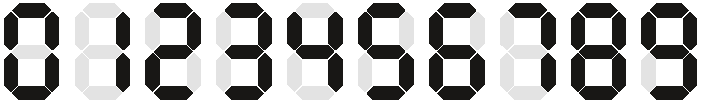
\includegraphics{C21-1}}
\newline
Greg chooses three different digits. In total, his digits have 5 horizontal segments and 10 vertical segments. What is the sum of his three digits?}
{9}{10}{14}{18}{19}
{A}{0}
{Each digit has 0, 1, 2 or 3 horizontal segments, so the total of 5 can be obtained as \newline
$5=2+2+1$ or \newline
$5=3+1+1$ or \newline
$5=3+2+0$. \newline
However, the first option is not possible since only 0 has two horizontal segments.
The second option is not also possible, since only 4 and 7 have one horizontal segment, and the digits 4 and 7 have a total of 3+2=5 vertical segments, meaning the third digit would need to have 5 vertical segments and the maximum possible is 4. \newline

Therefore there must be 3, 2, and 0 horizontal segments in the digits. Only digit 1 has no horizontal segments and only digit 0 has two horizontal segments and they have six vertical segments between them.  Therefore the final digit has three horizontal segments and four vertical segments and so is digit 8.  Hence, the sum of the digits is $8+0+1=9$.}

\problemID{22}{20248}{China}%
\problemRating{C}{5}{G}%
\Problem{Tarek wants to shade two further squares on the diagram shown so that the resulting pattern has a single axis of symmetry.  In how many different ways can he complete his pattern?
\newline
\centerline{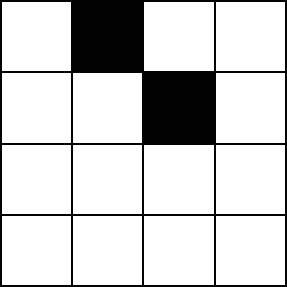
\includegraphics{C22-1}}}
{2}{3}{4}{5}{6}
{E}{0}
{The single axis of symmetry can be horizontal, vertical, diagonal from top left to bottom right and diagonal from bottom left to top right.  In the first three cases, Tarek can only shade two further squares in one way to give a symmetrical pattern.  However, in the final case, there are three possible ways to complete a symmetric pattern.  Hence, Tarek can complete his pattern in $1+1+1+3=6$ different ways.}

\NSidePictureEPS[scale=1.4]{C23-1}{\problemID{23}{20249}{Catalonia}%
\problemRating{C}{5}{G}%
\Problem{The diagram shows three semi-circles inside a rectangle.  The middle semi-circle touches the other two semi-circles which, in turn, each touch a shorter side of the rectangle.  The largest semi-circle also touches one of the longer sides of the rectangle.  The shortest distances from that side of the rectangle to the other two semi-circles are 5 cm and 7 cm respectively, as shown.  What is the perimeter, in cm, of the rectangle?}
{82}{92}{96}{108}{120}
{B}{0}
{Let $h \mathrm{cm}$ be the length of the unknown side of the rectangle. Therefore the radii of the three semi-circles, in cm, are $h$, $h-5$ and $h-7$. Therefore, by considering the longer side of the rectangle, we have  $2( h + h - 5 + h - 7) = 36$. This has solution $h= 10$.  Therefore the perimeter of the rectangle, in cm, is $2\cdot (36 + 10) = 92$.}}

\problemID{24}{20250}{China}%
\problemRating{C}{5}{N}%
\Problem{A group of 50 students sit in a circle.  They throw a ball around the circle.  Each student who gets the ball throws it to the 6th student sitting anti-clockwise from where they are sitting, who catches it.  Freda catches the ball 100 times. 
In that time, how many students never get to catch the ball?}
{0}{8}{10}{25}{40}
{D}{0}
{In order for a student to receive the ball again after passing it on, the ball must bypass a multiple of 50 students. As the ball is catched by every 6th student, it must also have bypassed a multiple of 6 students at any given time. Therefore, the ball must bypass 150 (the LCM of 50 and 6) students for the first student to receive the ball again. Before this occures, the ball has been passed to 150/6=25 students and we can be sure that no two students are the same because this would take at least 150 passes. After the first student receive the ball again and start passing it around for the second time, the passing pattern repeat itself and the same 25 players will get the ball again, meaning the other 25 players will never touch the ball.}

\NSidePictureEPS{C25-1}{\problemID{25}{20251}{Turkey}%
\problemRating{C}{5}{A}%
\Problem{Donggyu wants to complete the diagram so that each box in the middle and top rows will contain the product of the values in the two boxes below it and each box contains a positive integer.  He wants the value in the top box to be 720.\newline
How many different values can the integer $n$ take?}
{1}{4}{5}{6}{8}
{D}{0}
{Let $a$ and $b$ be the missing values in the boxes in the left-hand side and right-hand side of the bottom row respectively.  Therefore the values in the boxes in the middle row are $an$ and $bn$ and the value in the top row is $abn^2$.  However, we are told this value is 720 and hence $abn^2 = 720$.   Hence $n$ is a square factor of 720.  Now $720=1  \times 2 \times 2  \times 2  \times 2  \times 3 \times 3  \times 5$ and hence $n = 1, 2, 3 ,4, 6$ or $12$.}}

\problemID{26}{20252}{Hungary}%
\problemRating{C}{5}{N}%
\Problem{Farmer Fi is selling chicken and duck eggs.  She has baskets holding 4, 6, 12, 13, 22, and 29 eggs. Her first customer buys all the eggs in one basket.  Fi notices that the number of chicken eggs she has left is twice the number of duck eggs.  How many eggs did the customer buy?}
{4}{12}{13}{22}{29}
{E}{0}
{Fi had a total of $4 + 6 + 12 + 13 + 22 + 29 = 86$ eggs. After selling one basket, Fi notices that the number of chicken eggs she has left is twice the number of duck eggs.  Hence, the total number of eggs she has left is a multiple of 3.   Since 86 leaves a remainder of 2 when divided by 3, the number of eggs she sold also has a remainder of 2 when divided by 3.  Of the numbers of eggs in the different baskets, only 29 leaves a remainder of 2 when divided by 3.  Hence the customer bought 29 eggs.}

\problemID{27}{20253}{Belarus}%
\problemRating{C}{5}{G}%
\Problem{Three angles $\alpha,$ $\beta$ and $\gamma$ are marked on squared paper, as shown. What is the value of $\alpha+\beta+\gamma?$ \newline
\centerline{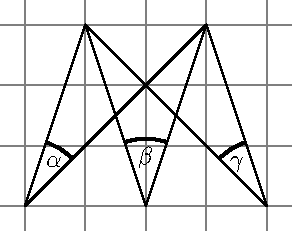
\includegraphics{C27-1}}}
{$60^\circ$}{$70^\circ$}{$75^\circ$}{$90^\circ$}{$120^\circ$}
{D}{0}
{The diagram shows a triangle with angles equal to $\alpha$, $\beta + \gamma$ and $90^\circ$.  Hence $\alpha+\beta+\gamma = 90^\circ$. 
\newline 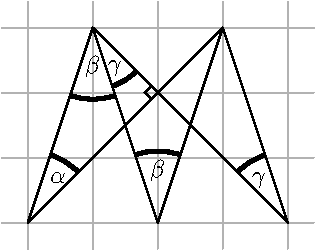
\includegraphics{C27-2}}

\problemID{28}{20254}{Greece}%
\problemRating{C}{5}{L}%
\Problem{Captain Flint asked four of his pirates to write on a piece of paper how many gold, silver and bronze coins were in the treasure chest.  Their responses are shown in the diagram but unfortunately part of the paper was damaged. Only one of the four pirates told the truth. The other three lied in all their answers.  The total number of coins is 30.  Who told the truth?
\newline\centerline{\includegraphics{C28-1F}}}
{Tom}{Al}{Pit}{Jim }{we cannot be sure}
{B}{0}
{Suppose Tom told the truth.  Then, since the total number of coins is 30, his response for gold coins would be $30-9-11 = 10$.  However, this is the same as Pit's response for gold coins and since the three pirates who lied, lied in all three of there answers, this is not possible.\newline
Now suppose Pit told the truth.  His response for silver coins would be $30-10-10 = 10$ but this is the same as Jim's response and so is not possible. \newline
Next suppose Jim told the truth.  His response for bronze coins would be 11 but this is the same as Tom's response and so is not possible.\newline
Therefore, since none of Tom, Pit or Jim told the truth, only Al can have told the truth.  His missing response for silver coins would be 11 and it can be seen that none of his answers match any of the other pirate's answers.}

\problemID{29}{20255}{Moldova}%
\problemRating{C}{5}{A}%
\Problem{Alex drives from point $A$ to point $B$, then immediately returns to $A$.  Bob drives from point $B$ to point $A$, then immediately returns to $B$.  They travel on the same road, start at the same time and each travels at a constant speed.   Alex's speed is three times Bob's speed. They pass each other for the first time 15 minutes after the start. How long after the start will they pass each other for the second time?}
{20 min}{25 min}{30 min}{35 min}{45 min}
{C}{0}
{Let $v_A$ and $v_B$ be Alex's speed and Bob's speed respectively. Assume boys meet for the first time in point $M$. Since $v_A=3v_B$, then $AM=3  BM$. Each boy covered his distance in 15 min. Since $v_A/v_B >2$, the second meeting took place before Bob reached $A$, assume in point $N$. Between meetings, Alex covered the distance $MB+BM+MN$, Bob covered the distance $MN$. Since $MB+BM+MN=3   MN$, we have $MB=MN$. Thus, Bob covered from the start till the second meeting the distance $BM+MN=2  BM$ in $2 \times 15=30$ min.}

\NSidePictureEPS{C30-6}{\problemID{30}{20256}{Hong Kong}%
\problemRating{C}{5}{G}%
\Problem{In the pentagon $ABCDE$, $\angle A =\angle B = 90^\circ$, $AE = BC$ and $ED = DC$.  Four points are marked on $AB$ dividing it into five equal parts. Then perpendiculars are drawn through these points, as shown in the diagram. The dark shaded region has an area of 13 cm$^2$ and the light shaded region has an area of 10 cm$^2$.  What is the area, in cm$^2$, of the entire pentagon?}
{45}{47}{49}{58}{60}
{A}{0}
{Since $\angle A =\angle B=90^\circ $ and $AE=BC$, $ABCE$ is a rectangle. If P is midpoint of  $AB$, the pentagon $ABCDE$ is axisymmetric. 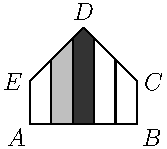
\includegraphics{C30-1}
\newline Draw the lines $FG$, $HI$ and $JK$ these are parallel to $AB$.
Lets look at the areas of the given figures:
\newline \includegraphics{C30-2} \includegraphics{C30-3} \includegraphics{C30-4} \includegraphics{C30-5}
\newline So, the area of the pentagon $= 2 \times (4+2) + 2 \times 10 + 13= 45$.}}


\end{document}